\begin{quote}
    \textit{``Is this clear? Now go home and prove it.'' --Jorge Santos, on the Penrose singularity theorem}
\end{quote}
We stated an important theorem last time, and we'll use it to prove something great.
%one of the few theorems I know that uses elementary fundamental mathematics to deduce something so physical.

\begin{thm}[Penrose singularity theorem (1965)]
    Let $(\cM,g)$ be globally hyperbolic with a non-compact Cauchy surface $\Sigma$. Assume the Einstein equations and the null energy condition hold, and that $\cM$ contains a trapped surface $T$. Let $\theta_0 < 0$ be the maximum value of $\theta$ on $T$ for both sets of null geodesics orthogonal to $T$. Then at least one of these geodesics is future-directed inextendible and has a finite length no greater than $2/|\theta_0|.$
\end{thm}
%Is this clear? Now go home and prove it.
\begin{proof}
    We will prove this by contradiction. Assume that all inextendible null geodesics orthogonal to $T$ have affine length greater than $2/|\theta_0|$. By the Raychaudhuri equation, we saw that along any of these geodesics, we will have $\theta\to-\infty$. Hence a point conjugate to $T$ within affine parameter distance no greater than $2/|\theta_0|$.
    
    It's time to use our theorem from last time. Let $p\in \dot J(T), p \notin T$. From Thm. \ref{surfaceconjugatepoints}, we know that $p$ lies on a future-directed null geodesic $\gamma$ starting from $T$ which is orthogonal to $T$ and has no point conjugate to $T$ between $T$ and $p$. It follows that $p$ cannot lie beyond the point on $\gamma$ conjugate to $T$ on $\gamma$.
    
    Therefore $\dot J^+(T)$, the topological boundary of the causal future of $T$, is a subset of a compact set consisting of the set of points along the null geodesics orthogonal to $T$ with affine parameter less than or equal to $2/|\theta_0|$. But $\dot J^+(T)$ is a boundary, hence closed, which implies that $\dot J^+(T)$ is in fact compact.%
        \footnote{That is, a closed subset of a compact set is compact.}
    
    Now recall that $J^+(T)$ is a (sub)manifold, which implies that it cannot have a boundary.%
        \footnote{Some people make a distinction between manifold with boundary and manifold without boundary. We won't bother here, and assume that a manifold just looks like $\RR^n$ everywhere.}
    In addition, we said that $\Sigma$ is a non-compact Cauchy surface. Therefore pick a timelike vector field $T^a$ (we are free to do this since our manifolds are time-orientable). By global hyperbolicity, integral curves of $T^a$ intersect $\Sigma$ exactly once. Notice that they will intersect $\dot J^+(T)$ at most once because $\dot J^+(T)$ is achronal (otherwise, two points would be connected by a timelike curve). This defines a continuous one-to-one map $\alpha:\dot J^+(T) \to \Sigma$, as illustrated in Fig. \ref{fig:jplushomeomorphism}. In particular this is a homeomorphism between $\dot J^+(T)$ and $\alpha(\dot J^+(T))\subset \Sigma$. Since the former is a closed set, so is the latter.
    
    Now $\dot J^+(T)$ is a 3D submanifold, and hence for any $p\in \dot J^+(T)$, we can find a neighborhood $V$ of $p$ with $V\subset \dot J^+(T)$. Then $\alpha(V)$ gives a neighborhood of $\alpha(p)$ in the image $\alpha(\dot J^+(T))$. Hence the latter set is open in $\Sigma$.
    
    Since $\alpha(\dot J^+(T))$ is both open and closed in $\Sigma$, it must be the entire set,
    \begin{equation*}
        \alpha(\dot J^+(T))=\Sigma.
    \end{equation*}
    But we showed that $\alpha(\dot J^+(T))$ was compact, and by assumption $\Sigma$ was noncompact. Therefore we have reached a contradiction.
\end{proof}

\begin{figure}
    \centering
    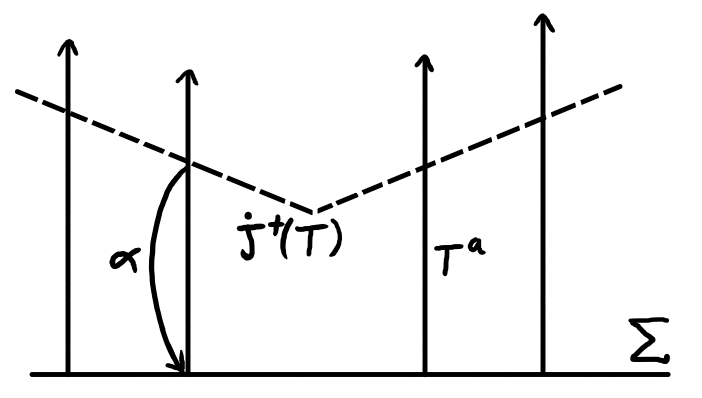
\includegraphics[width=0.5\textwidth]{2019/02/20190222_jplushomeomorphism.png}
    \caption{An illustration of the homeomorphism between $\dot J^+(T)$ and $\Sigma$. By following the timelike curves which are the integral curves of $T^a$ (the time-orientation of our spacetime) backwards from $\dot J^+(T)$ to some subset of $\Sigma$, we get a continuous one-to-one map $\alpha: \dot J^+(T)\to \Sigma$.}
    \label{fig:jplushomeomorphism}
\end{figure}

It seems like we haven't quite gotten the result we were promised. Penrose requires a trapped surface, and maybe it's the case that trapped surfaces never form. However, due to an incredible result by Christodoulou, it turns out that trapped surfaces do form when you scatter enough gravitons, at least in Minkowski backgrounds. Moreover, there's the notion of Cauchy stability, i.e. given initial conditions that lead to a trapped surface, we can perturb them, solve the Einstein equations, and see how the new solution depends on the perturbation. It turns out that generically, perturbed spacetimes which had trapped surfaces before perturbation do still feature trapped surfaces, and we can do analytic calculations in spherical symmetry which do have trapped surfaces in them. Numerically, trapped surfaces turn up all the time. Therefore life is not so bad. Trapped surfaces are basically generic and so singularities are generic. QED.

\subsection*{Asymptotic flatness}
We have discussed asymptotic flatness in the context of initial conditions. What does it mean for a spacetime to be asymptotically flat? To understand this, we'll need the notion of \term{conformal compactification}.

Given a spacetime $(\cM,g)$, we can define a new metric
\begin{equation}
    \bar g= \Omega^2 g.
\end{equation}
In particular, we can choose $\Omega$ such that the resulting spacetime $(\cM,\bar g)$ is extendible into $(\bar \cM,\bar g)$. That is, $M$ is a proper subset of $\bar \cM$. Note that since $\Omega^2$ is non-negative (generally, positive), the causal structure of the spacetime will be respected by this transformation. Spacelike separations in $g$ will also be spacelike in $\bar g$, and so on. 

Let's start with Minkowski space. Let $(\cM,g)$ be Minkowski in spherical coordinates,
\begin{equation}
    g = -dt^2 +dr^2 +r^2 d\omega^2,
\end{equation}
where we denote the round 2-sphere metric by $\omega$ to avoid confusion with the conformal factor $\Omega$. Define advanced and retarded (light cone) coordinates
\begin{equation}
    u=t-r,\quad v=t+r.
\end{equation}
Under this change of coordinates, we get the metric
\begin{equation}
    g=-dudv +\frac{1}{4}(u-v)^2 d\omega^2.
\end{equation}
Now we'll make a somewhat stranger change of coordinates,
\begin{equation}
    u=\tan p, \quad v=\tan q
\end{equation}
where in the $(p,q)$ coordinates, $-\pi/2 < p \leq q < \pi/2$. Substituting back into the metric, we get something that looks kind of weird. It's
\begin{equation}
    g=\frac{1}{(2\cos p \cos q)^2} \bkt{-4 dpdq + \sin^2(q-p)d\omega^2}.
\end{equation}
Notice that this denominator diverges when $q\to \pi/2$, so this suggests to us a very natural choice of conformal factor $\Omega$. It's just
\begin{equation}
    \Omega=2\cos q \cos p,
\end{equation}
which gives us a new metric
\begin{equation}
    \bar g=-4 dpdq + \sin^2(q-p)d\omega^2 = \Omega^2 g.
\end{equation}
Finally, make the coordinate transformation
\begin{equation}
    T=q+p\in (-\pi,\pi), \quad \chi=q-p \in [0,\pi).
\end{equation}
What we get is the metric
\begin{equation}
    \bar g= -dT^2 +\underbrace{d\chi^2 +\sin^2 \chi d\omega^2}_{S^3},
\end{equation}
which looks very much like the Einstein static universe! Except there's a little caveat-- the coordinate ranges mean that we don't get the whole of the cylinder. In fact, the range of $\chi$ also depends on $T$. An illustration of this appears in Fig. \ref{fig:reallesudiagram}.
\begin{figure}
    \centering
    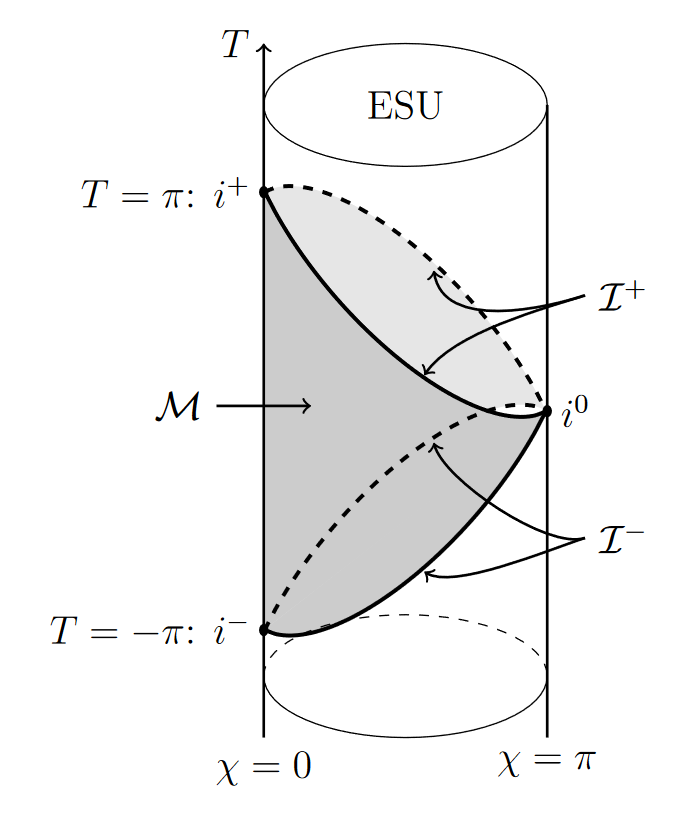
\includegraphics{2019/02/20190222_reallesudiagram.png}
    \caption{The patch of the Einstein static universe conformally equivalent to Minkowski space. The ESU has the topology of $\RR\times S^3$, so we suppress two of the angular coordinates to draw this as a cylinder instead, $\RR\times S^1$, where the $T$ direction runs vertically and one of the angular coordinates (say, $\chi$) runs around the circumference of the cylinder. Also indicated are future/past timelike infinity $i^\pm$, future/past null infinity $\mathcal{I}^\pm$, and spacelike infinity $i^0$. Image credit to Prof. Reall's  \href{http://www.damtp.cam.ac.uk/user/hsr1000/black_holes_lectures_2016.pdf}{Black Holes notes}, \textsection 5.1.
    }
    \label{fig:reallesudiagram}
\end{figure}
%That's it. This is my best, guys.
%We get a diagram that looks like the following:
Moreover, by projecting down into the $T$-$\chi$ plane (so that each point represents a 2-sphere), we get the Penrose diagram for Minkowski space, seen in Fig. \ref{fig:reallminkowskipenrose}. Penrose diagrams are very good for radial motion, but they come at the slight cost of hiding all angular motion behind our projection. In addition, note that under this projection, the points $(T=T_0,\chi=+\chi_0)$ and $(T=T_0,\chi=-\chi_0)$ are collapsed to the same point. I emphasize that there is nothing special about $\chi=0$ in Minkowski space-- it is utterly non-singular. This is just a quirk of our projection, taking advantage of the spherical symmetry of our spacetime.

\begin{figure}
    \centering
    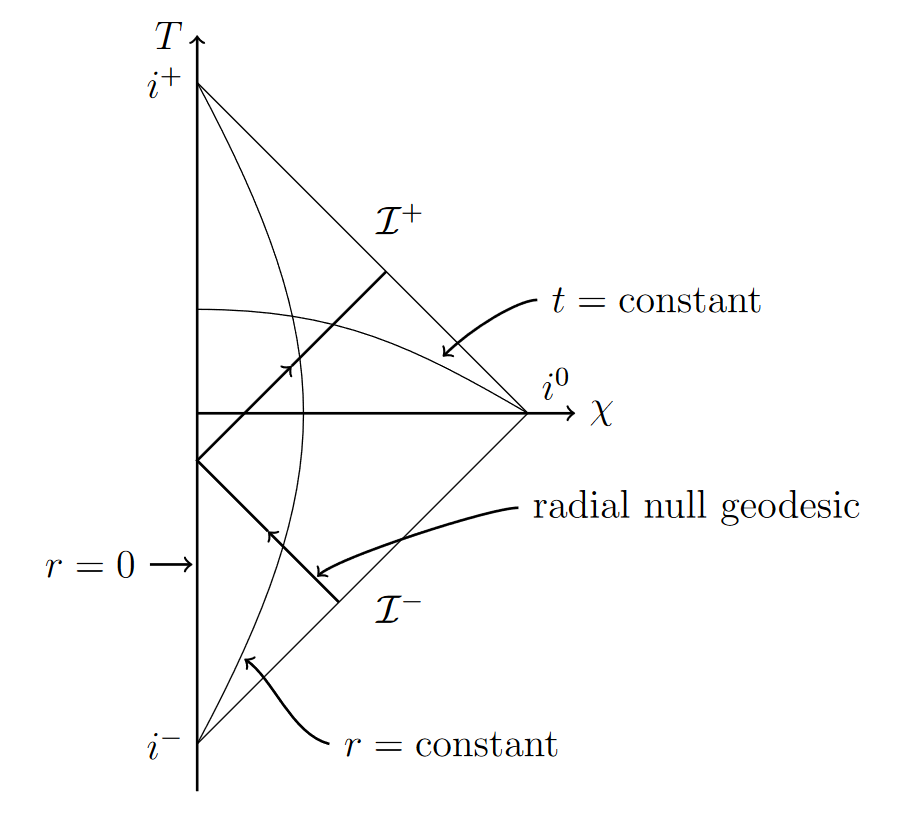
\includegraphics{2019/02/20190222_reallminkowskipenrose}
    \caption{The Penrose diagram for Minkowski space. Note that the radial null geodesic drawn is not ``reflecting'' off anything; there is nothing special about $r=0$ in Minkowski space. The geodesic simply passes through $r=0$ and then proceeds back out to larger values of $r$ as it heads towards future null infinity, $\mathcal{I}^+$. Image credit to Prof. Reall's  \href{http://www.damtp.cam.ac.uk/user/hsr1000/black_holes_lectures_2016.pdf}{Black Holes notes}, \textsection 5.1.}
    \label{fig:reallminkowskipenrose}
\end{figure}

It's also important to notice that we've introduced an unphysical, extendible metric $\bar g$. Minkowski space itself is inextendible, but after a conformal transformation we got a subset of the Einstein static universe (where this subset is very clearly extendible). Moreover, conformal transformations preserve the causal structure of spacetime, so we've found a very nice way to illustrate the causal structure of a spacetime. In the next lecture, we'll look at the solutions to wave equations living in curved spacetime.